\documentclass[a4paper]{scrartcl}
\usepackage[utf8]{inputenc}
\usepackage[english]{babel}
\usepackage{graphicx}
\usepackage{lastpage}
\usepackage{pgf}
\usepackage{wrapfig}
\usepackage{fancyvrb}
\usepackage{fancyhdr}
\pagestyle{fancy}

\usepackage[backend=bibtex, citestyle=numeric-comp, bibstyle=ieee]{biblatex}
\addbibresource{ref.bib} % The file containing our references, in BibTeX format
\usepackage{hyperref}
\usepackage{listings}
\usepackage{subcaption}

% Create header and footer
\headheight 27pt
\pagestyle{fancyplain}
\lhead{\footnotesize{Internet Applications, ID1354}}
\chead{\footnotesize{Tasty Recipes with HTML and CSS}}
\rhead{}
\lfoot{}
\cfoot{\thepage\ (\pageref{LastPage})}
\rfoot{}

% Create title page
\title{Tasty Recipes with HTML and CSS}
\subtitle{Internet Applications, ID1354}
\author{Julius Recep Colliander Celik - jcelik@kth.se}
\date{\today}

\begin{document}

\maketitle

%\section*{Tips for Report Writing}
%\textbf{REMOVE THIS SECTION BEFORE SUBMITTING THE REPORT.}\\
%
%\noindent \textit{The target audience has exactly the same skills as the author, except they do not know anything at all about the specific program described in the report.} \\
%
%Consider the following:
%
%\begin{itemize}
%  \item \textbf{The report must be \textit{centered around the requirements}. Which are they (Introduction), how did you work to meet them (Method), what is the solution that meets them (Result), and how can you be sure they are met (Discussion). This is the IMRaD method.}
%
%  \item \textbf{The report must show that you have done the work yourself and that you have understood what you have done. Both of these goals are met by carefully explaining the source code.}
%
%  \item Is spelling and grammar correct? Is spoken language avoided?
%
%  \item Does the report have a good structure with sections, subsections and paragraphs?
%
%  \item Is the solution clearly explained? Will the reader understand the program? What would you yourself want to know if you read about the program, is that included in the report?
%
%  \item Is the solution analyzed and evaluated? Are important properties of the program explained? Should there have been more extensive evaluation?
%
%  \item Is the text clarified with images and/or other figures, and with links to the code in your Git repository? Remember that all figures (images, tables, graphs, code listings, etc) shall be numbered and have a short explaining text.
%\end{itemize}

\section{Introduction}

A web site for sharing tasty recipes was created. The goal was to create a web site using only HTML and CSS, following halve of the heuristics of user design, as well as considering accessibility, and preferably being responsive by adapting the web site to different screen sizes. To ensure consistency a CSS reset style sheet had to be used, and to ensure good code quality all files created had to be pass the W3C validations.

The web site created contained of four pages. One home page, two recipe pages, and one calendar page. Every page had to be accessible from any other page, which is why a navigation menu was recommended. To view the website it is publicly available on the link \href{https://github.com/juliuscc/kth-id1354/tree/master/homework-1}{https://github.com/juliuscc/kth-id1354/tree/master/homework-1}.

\section{Literature Study}

The web page w3schools is a web page with extensive information about HTML, CSS and many other web technologies. The web page w3schools was used for basic CSS reference \cite{RefsnesData}. For reference of CSS Flexbox and CSS Grid the complete guides from CSS-Tricks was used \cite{Coyier,Coyiera}. 

For design inspiration, the calendar is visually based on another calendar. A calendar created using the framework Semantic UI was openly shared and was the basis for creating the calendar on the Tasty Recipes web site \cite{Nijin39} . As I have been mostly fluent in HTML and CSS, for the past 4 years prior to this assignment, no other resources were necessary.

\section{Method}
This chapter is divided into two parts. The first part (Chapter \ref{method:development}) explains the tools used and the development environment. It also describes how the web site was publicly published. The second part (Chapter \ref{method:evaluation}) explains how the web page was evaluated. The web site was mostly manually evaluated, however browser compatibility and code validity is discussed in this chapter.

\subsection{Development environment}
\label{method:development}

The text editor used was Visual Studio Code. This decision was based on personal preference, as well as it being the most popular development environment \cite{Stackoverflow}. I considered using SASS with an SCSS syntax, or PostCSS as it helps with structuring projects. After consideration I choose to use only pure HTML and CSS as the project is very small and simple. To keep a good structure on my CSS I used the Block Element Modifier (BEM) methodology. It is a very simple naming methodology that results in very elegant code \cite{Starkov}.

Of course I used a CSS reset style sheet. I used Normalize.css as I have used it before successfully. It is very lightweight and primarily aims at fixing browser bugs and inconsistent behavior, while preserving useful browser defaults. It is used by ``[...] Twitter, TweetDeck, GitHub, Soundcloud, Guardian, Medium, GOV.UK, Bootstrap, HTML5 Boilerplate, and many others'' \cite{Gallagher}.

To deploy the web site I use GitHub Pages, and use CloudFlare for CDN cache and redirection so that the url \texttt{https://receps-recept.com} results in the web site hosted on GitHub Pages being received. For automatic continuous deployment I use Travis CI. For local development I used Browsersync to refresh my browser every time a file was changed. It enabled me to have the web site next to my code and not have to manually refresh the web page every time I made a change in the code.

\subsection{Evaluation}
\label{method:evaluation}

To evaluate  the validity of my code I used the W3C Markup Validation Service. It catched one error where I downloaded a font with the link:\\ \small{\texttt{https://fonts.googleapis.com/css?family=Kaushan+Script|Permanent+Marker|Lato}} where the character \texttt{|} is not allowed. I changed that to \texttt{\%7C}.

I tested my web site on the following browsers:
\begin{itemize}
	\item Google Chrome - Mac OS X
	\item Firefox - Mac OS X
	\item Safari - Mac OS X
	\item Google Chrome - iOS 12
	\item Opera Mini - iOS 12
	\item Safari - iOS 12
\end{itemize}

This was to ensure that the web site performed consistently over multiple browsers. On the computer I tested both normal view and mobile view in Firefox. The most interesting browser on the list is Opera Mini that is a browser that lacks a large amount of modern features, and purposely ignores certain web features to save battery, internet bandwidth and perform better. It is not always required for the web site to look exactly the same on Opera Mini as it would be limiting for other users, however it is important that the website still is usable on Opera Mini. Internet Explorer and Internet Edge could not be tested as no compatible device was available. However Internet Edge is a browser that often have the latest features, despite Microsoft's history with Internet Explorer being a worse browser than the competitors.

\section{Result (and html head)}

\textbf{This section explains \textit{the result} of what you did.} \\

\noindent Present the solution. Explain your code and prove that it meets the requirements. It is very important to \textit{state each requirement that is met} and explain \textit{how you met it}. It is also important to include links to your code in your Git repository, user interface screen-shots, see Figure \ref{fig:ui}, and other figures to illustrate your reasoning. Also remember that these figures must be referenced in the text.

\subsection{Project Structure}
The project uses the following file structure:

\begin{verbatim}
|---- icons
|   |---- bars-solid.svg
|   +---- times-solid.svg
|---- images
|   |---- blur-close-up-dairy-product-407041.jpg
|   |---- board-bunch-cooking-349609.jpg
|   +---- emiliano-vittoriosi-703094-unsplash.jpg
|---- calendar.html
|---- index.html
|---- meatballs.html
|---- normalize.css
|---- pancakes.html
+---- style.css
\end{verbatim}

\noindent
It contains four HTML-files which each correspond a page, two CSS style sheets where one is a CSS reset and the other is the web pages style, as well as icons and images.

\subsection{W3C validation and CSS Reset Style Sheet}
The HTML pages and the style sheet were all submitted to the W3C Markup Validation Service. All the four HTML-files and the CSS style sheet showed no errors or warnings. A CSS reset style sheet was used. Normalize.js was the reset style sheet used. It was added in the head before any other style sheets. All pages looked the same on all tested browsers.

\subsection{CSS}
The CSS is written with BEM methodology to make it easier to work with. For horizontal alignment i use mostly percentages to ensure that the web site always looks nice. I also use media queries to change the style based on screen size. Following is a small example of two block classes and their descendant elements and the modifier classes. It also shows that I use CSS Grid, box-shadows, transitions and media queries.

\begin{lstlisting}
/*
============== RECIPE LIST ==============
*/

.recipe-list {
	padding: 0 20%;
	padding-bottom: 25px;
}

.recipe-list__title {
	font-size: 30px;
}

.recipe-list__card-wrapper {
	display: grid;
	grid-template-columns: repeat(2, 1fr);
	grid-gap: 20px;
}

@media (max-width: 800px) {
	.recipe-list {
		padding: 0 8%;
		padding-bottom: 25px;
	}
	
	.recipe-list__card-wrapper {
		grid-template-columns: 1fr;
	}
}

/*
============== RECIPE CARD ==============
*/

.recipe-card {
	box-shadow: rgba(0, 0, 0, 0.5) 0px 3px 9px -4px;
	text-decoration: none;
	color: black;
	border-bottom: #ff5526 5px solid;
	
	transition: transform 0.2s, box-shadow 0.2s;
}

.recipe-card:hover {
	box-shadow: rgba(0, 0, 0, 0.5) 0px 10px 15px -4px;
	/* translateZ(0) forces hardware acceleration */
	transform: scale(1.01) translateZ(0);
}

.recipe-card__image {
	width: 100%;
	height: 400px;
	object-fit: cover;
}

@media (min-width: 800px) and (max-width: 1200px) {
	.recipe-card__image {
		height: 200px;
	}
}

.recipe-card__title {
	font-size: 25px;
	margin: 10px;
	margin-top: 5px;
}
\end{lstlisting}

\subsection{Index Page (design)}

The index page is shown in figure \ref{fig:index-page}. If the screen is smaller than 800px in width the web page changes design to the one shown in figure \ref{fig:index-page-mobile}. The primary changes are smaller margins, the grid has fewer columns, and the navigation bar becomes a collapsible and vertical navigation bar. Figure \ref{fig:mobile-nav} shows the navigation bar in the expanded state. It uses a hidden checkbox to trigger the state change. The text \textit{Menu} is a label that triggers a change in the checkboxes state.

\begin{figure}
	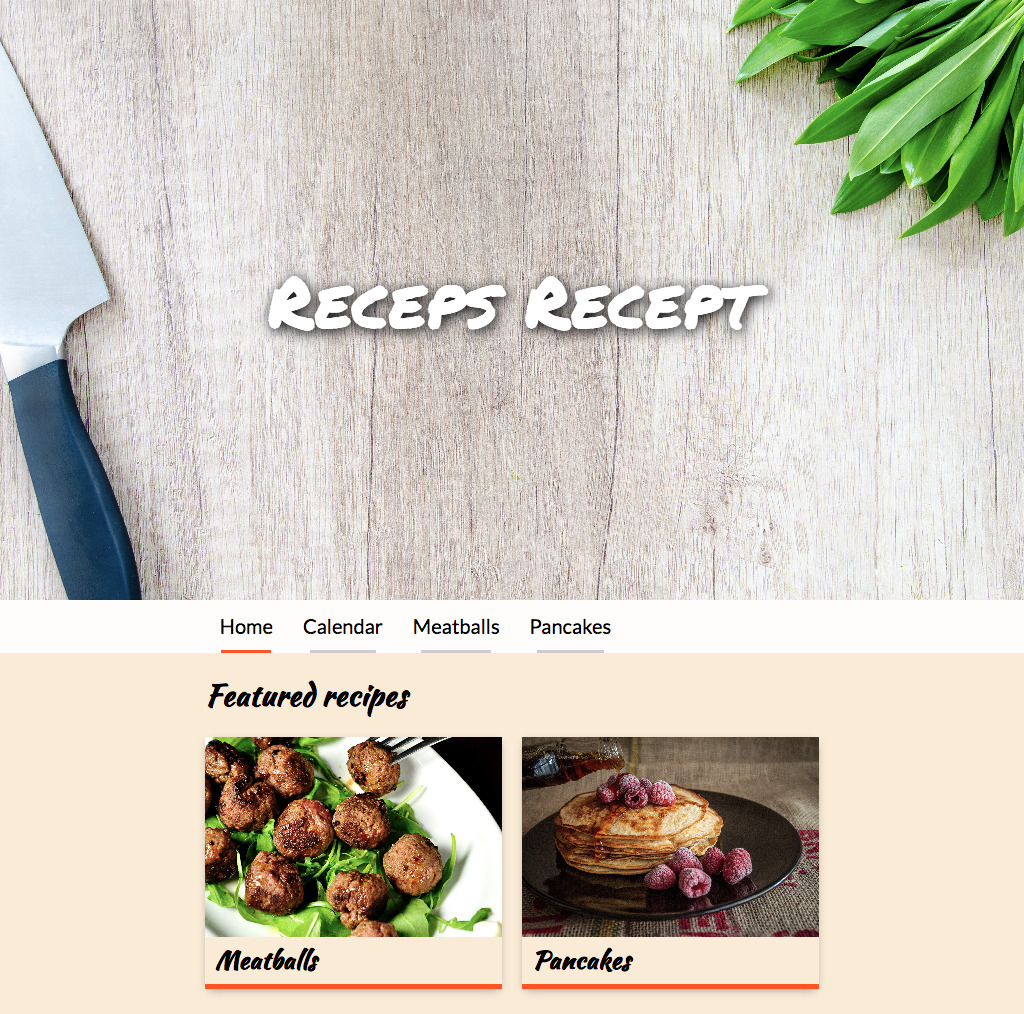
\includegraphics[width=\linewidth]{images/screenshot-index.jpg}
	  \caption{Index page (Desktop)}
	\label{fig:index-page}
\end{figure}

\begin{figure}
	\centering
	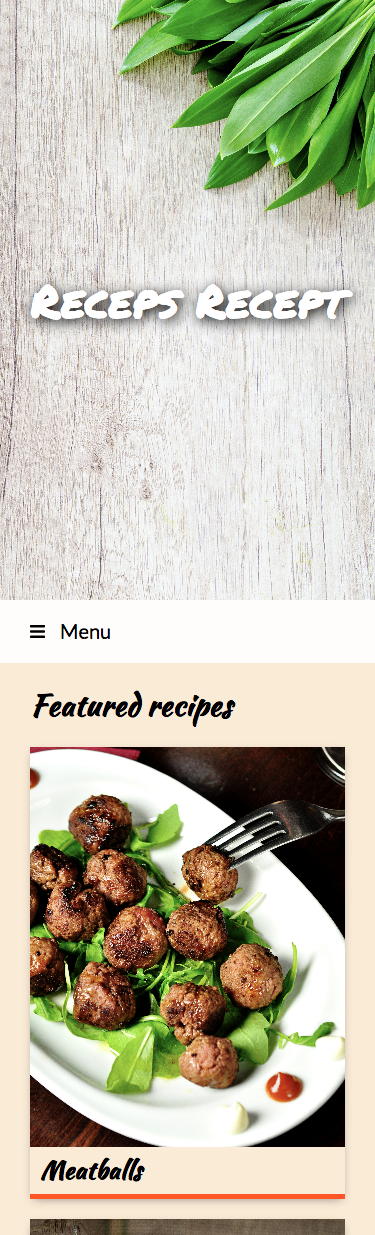
\includegraphics[height=\dimexpr\textheight-3\baselineskip-\parskip-.2em-\abovecaptionskip-\belowcaptionskip\relax]{images/screenshot-index-mobile.png}
	\caption{Index page (mobile)}
	\label{fig:index-page-mobile}
\end{figure}

\begin{figure}
	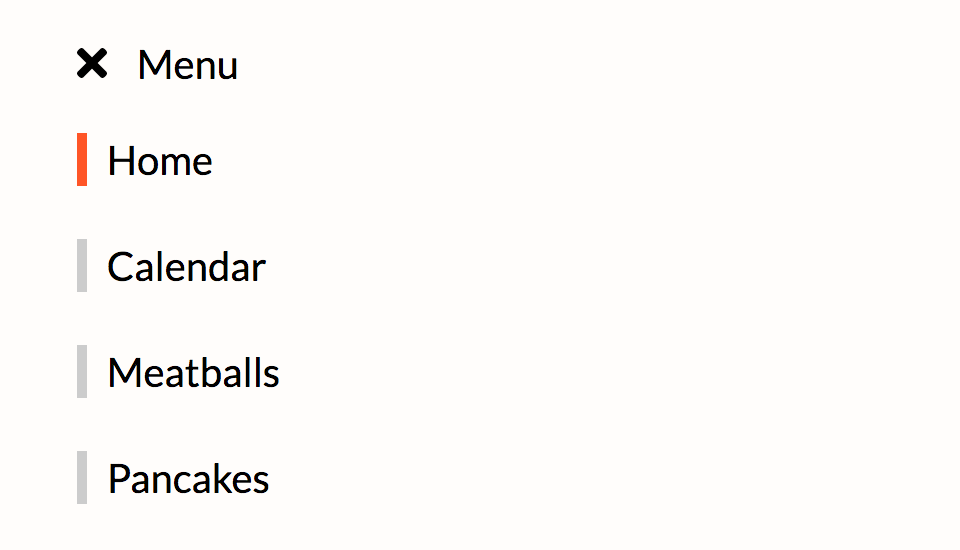
\includegraphics[width=\linewidth]{images/mobile-menu-expanded.png}
	\caption{Mobile navigation bar in expanded state}
	\label{fig:mobile-nav}
\end{figure}

\subsection{Calendar Page (design)}

As mentioned the calendar in the calendar page was inspired from another one. It was inspired on the design of a calendar created with Semantic UI. A comparison of the two is shown in figure \ref{fig:calendar-comparison}.

\begin{figure}
	\centering
	\begin{subfigure}[b]{0.45\linewidth}
		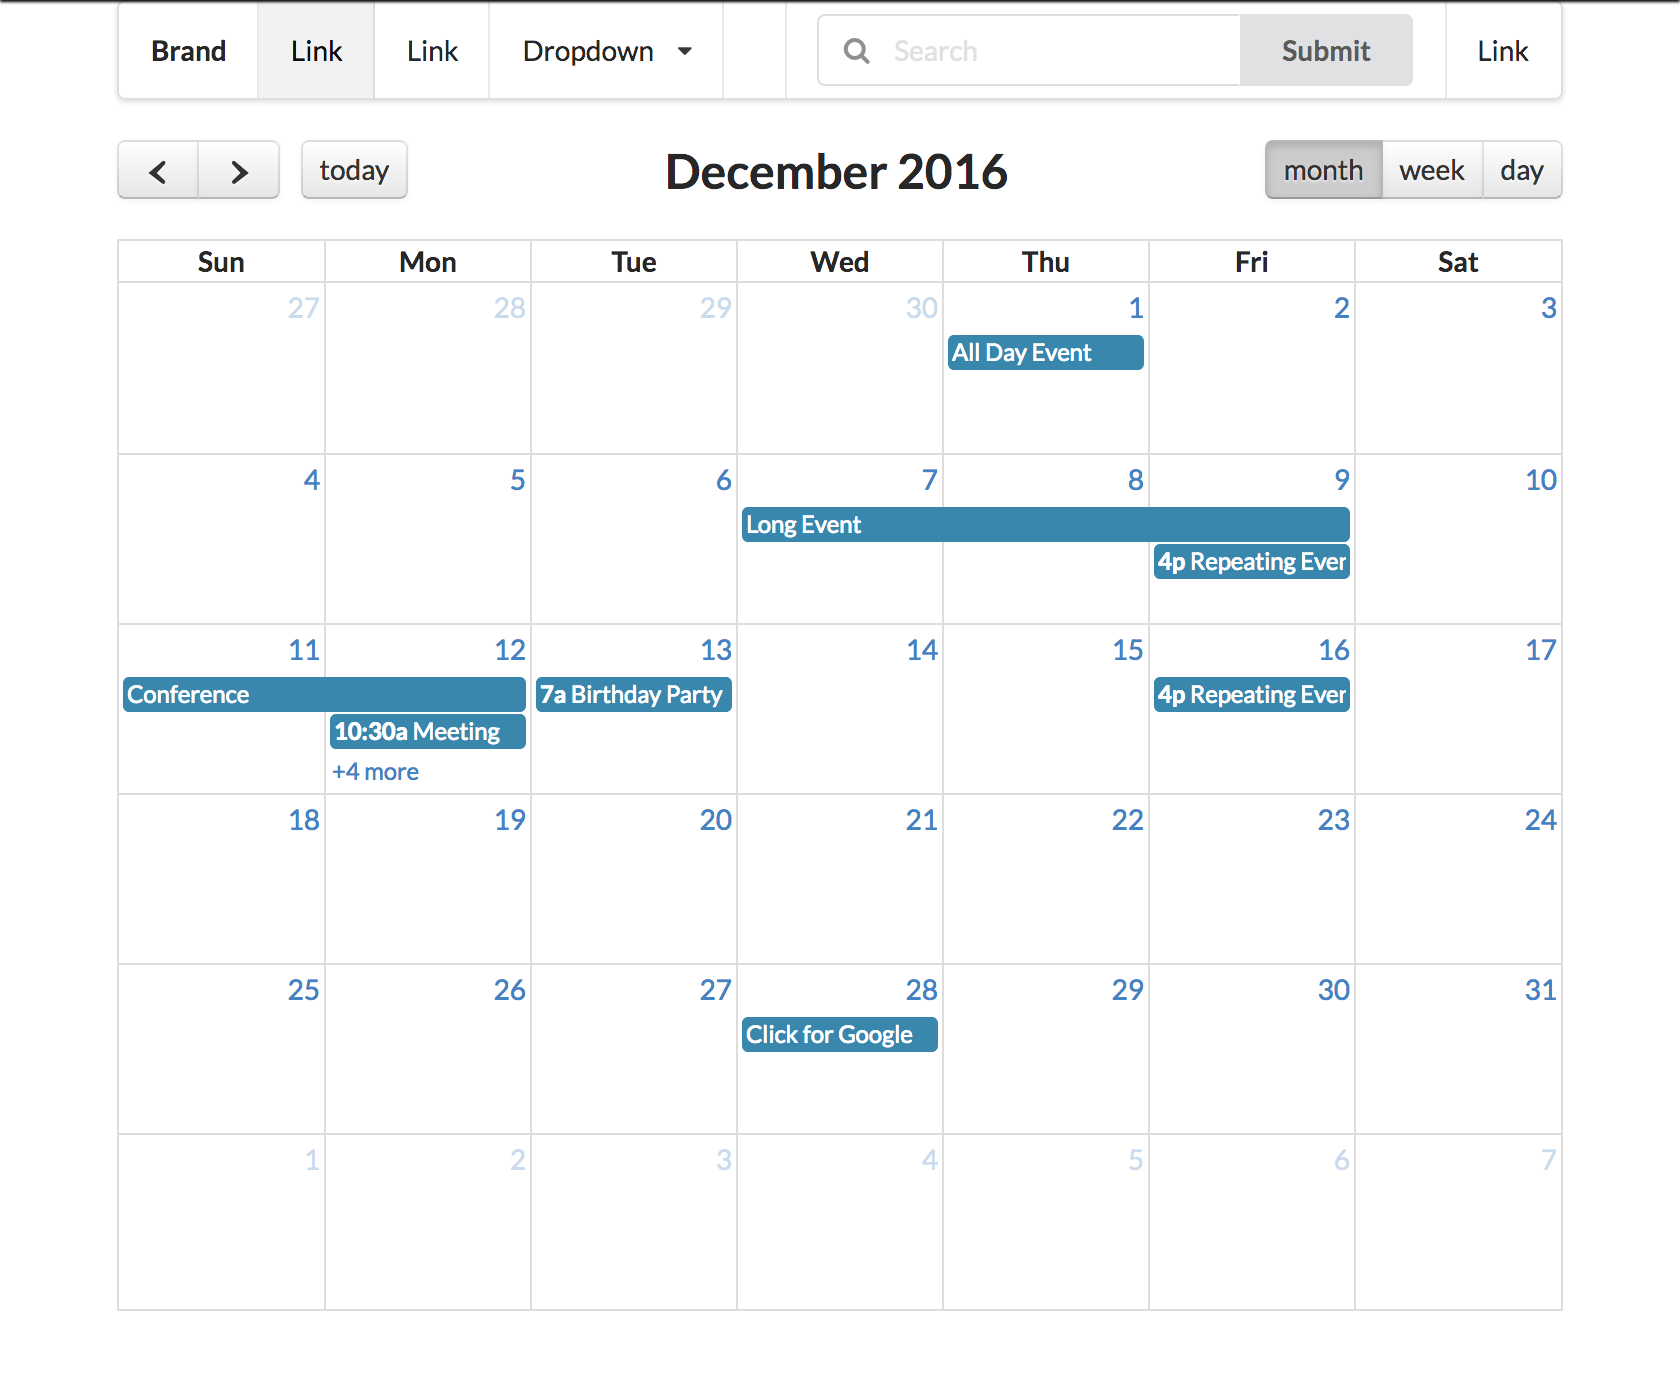
\includegraphics[width=\linewidth]{images/Semantic_UI-calendar.png}
		\caption{Semantic UI - Calendar}
	\end{subfigure}
	\begin{subfigure}[b]{0.45\linewidth}
		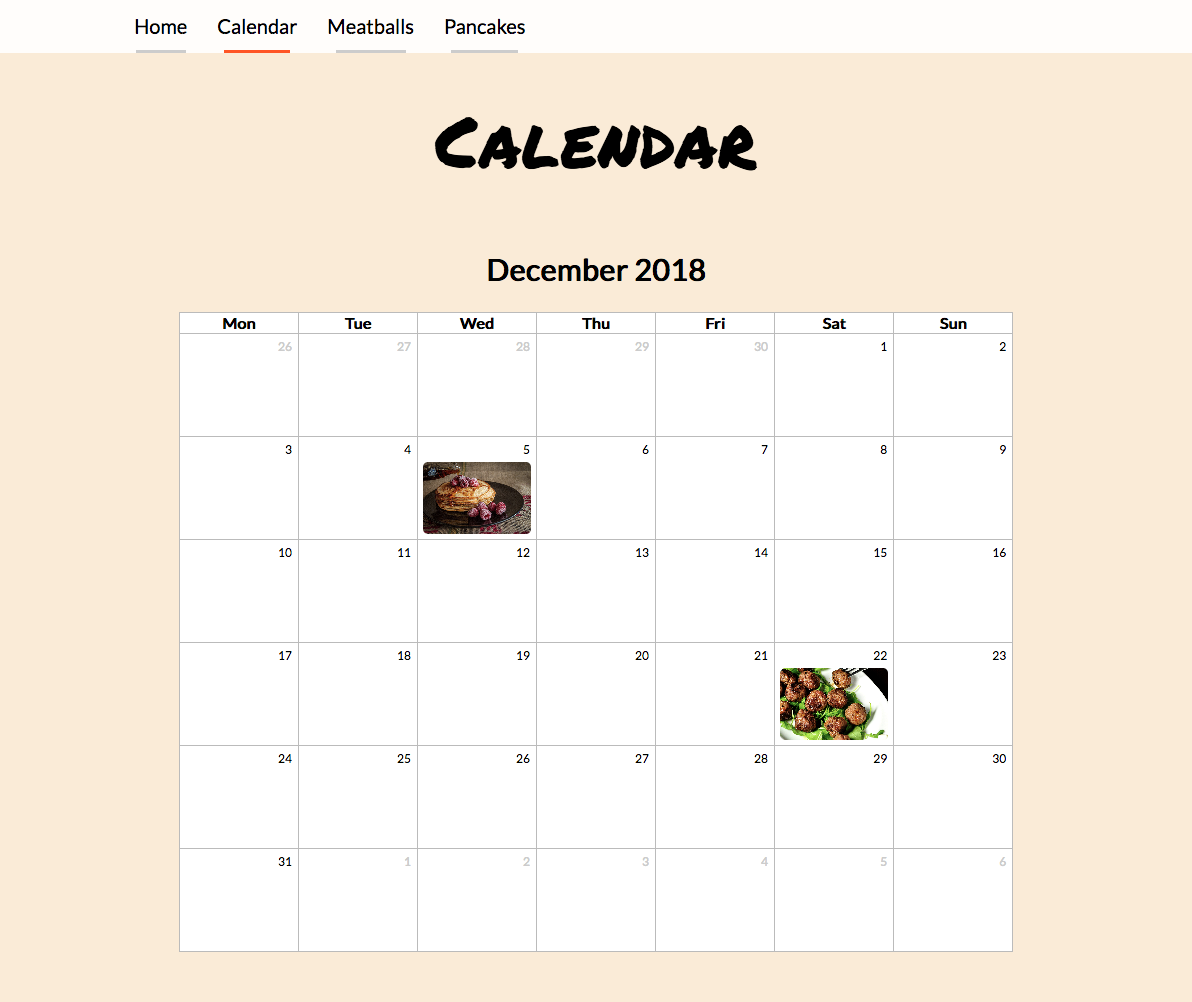
\includegraphics[width=\linewidth]{images/calendar.png}
		\caption{Receps Recept - Calendar}
	\end{subfigure}
	\caption{Calendar comparison}
	\label{fig:calendar-comparison}
\end{figure}

\subsection{Heuristics of user design}

Five of the ten basic heuristics for user interface design was considered.

\subsubsection{Visibility of system status}
The web page is mostly stateless. The only state is the state of the navigation bar when viewing the web page with a mobile device, or a device with a very small screen. The interaction is instant so the state is always visible. The state of the navigation bar can be collapsed or expanded, which is indicated with an icon.

\subsubsection{Match between system and the real world}
All of the user visible text is adapted to the users. All of the text has been proofread.

\subsubsection{Consistency and standards}

% 4. Consistency and standards.
% Navbarens position
% Navbaren ser dock likadan ut på varje sida. Det finns liknande element på mobil och desktop.
% Bara tre fonts används och de används alltid till samma sak

% 6.  Recognition rather than recall.
% Alla användarinteraktioner är tydliga. Man måste inte komma ihåg något för att hitta en sida man tidigare besökte då de alltid är lätta att hitta. Ingridienser, instruktioner och kommentarer är samlade på samma ställe.
% Bilder hjälper användare hitta rätt på första-sidan
% Bilder används i kalendern

% 8. Aesthetic and minimalist design.
% Menyn är collapsible när skärmen är mindre och informationsdensiteten är lägre, vilket leder till att varje elements viktighetsgrad måste värderas högre.
% Det finns inga överdrivna funktioner. Designen är simpel

\subsection{Responsiveness}

\subsection{Accessibility}


\section{Discussion}

\textbf{This section \textit{analysis} the result presented in the previous section.} \\

\noindent Summarize the requirements and \textit{clearly state which of them you have met}. What lessons have you learned and what problems did you face? How were the problems solved? Should you have done something differently?

\section{Comments About the Course}

Any comment(s) related to this course offering or to coming offerings is much appreciated. \textit{Please also tell approximately how much time you spent on the assignment}, including lectures and exercises. This is of great help for course evaluation.

\printbibliography[heading=bibintoc]

\end{document}
